\documentclass[a4paper, 11pt]{article}
\usepackage{comment} % enables the use of multi-line comments (\ifx \fi) 
\usepackage{lipsum} %This package just generates Lorem Ipsum filler text. 
\usepackage{fullpage} % changes the margin
\usepackage{tikz}
\usetikzlibrary{arrows,automata,positioning}
\usepackage[utf8]{inputenc}

\begin{document}
%Header-Make sure you update this information!!!!
\noindent
\large\textbf{Lenguajes Formales y Autómatas/Proyecto} \hfill \textbf{Integrantes del grupo:} \\
\normalsize INF - 154 \hfill Jhonatan Ismael Castro Rocabado\\
Profesora. Madelina Loza Soliz \hfill Fabiola Vanessa Aliaga Salvatierra\\
Periodo: Curso de Invierno 2016 \hfill Carlos Fernando Torrez Alanoca\\
\hfill Fecha: 27/7/2016 \\

\section*{Introducción}
Como vimos en las clases de lenguajes autómatas y formales, podemos asegurar que las gramáticas libres de contexto nos ayudan a la realización de varias aplicaciones como ser: "El lenguaje de las expresiones algebraicas" , "Sintaxis en los lenguajes de programación" , "Reglas Gramaticales en español". En el siguiente proyecto explicaremos de manera más profunda la realización de la primera aplicación:
"El lenguaje de las expresiones algebraicas".

Para realizar éste proyecto necesitamos saber definiciones básicas de lo que son las gramáticas libres de contexto y en especial el lenguaje que genera una gramática de contexto libre. 
Un lenguaje importante en la ciencia de la computación es de expresiones algebraicas válidas. Por simplicidad, el análisis se limita aqui a expresiones sencillas que pueden formarse con los operadores binarios: +, -,* y /, además de los signos de abrir y cerrar parentesis, y del identificador único a.
Por tanto, algunas de las caracteristicas omitidas son los operadores unarios, expresiones relativas a la notación funcional e identificadores más generales.
Muchas de esas caracteristicas podrían manejarse con mucha mas sencillez.
Una definición recursiva del lenguaje se basa en la observación que pueden formarse expresiones válidas al unir dos expresiones válidas con uno de los cuatro operadores o encerrar una expresión válida entre parentesis, además de que estas dos operaciones sirven para explicar todas las expresiones válidas, salvo el identificador unico a. Así pues, la forma más directa de obtener una gramática de contexto libre probablemente  sea el uso de las producciones:

S $\rightarrow$ S + S  $|$ S - S  $|$ S * S  $|$ S / S  $|$ (S)

De esa manera pueden evaluarse diversas derivaciones. 

En el siguiente proyecto presentaremos una gramática libre de contexto representado por un autómata finito que evalúa el lenguaje de expresiones algebraicas con su respectiva matriz de transiciones y el código fuente en java Script. 

\section*{Enunciado del Problema}
Realizar un autómata que acepte enunciados de operaciones algebraicas simples.

\section*{Autómata}

%%% First Automata
\subsection*{var++, var + var, var+=} % sub title

% code of the graphic
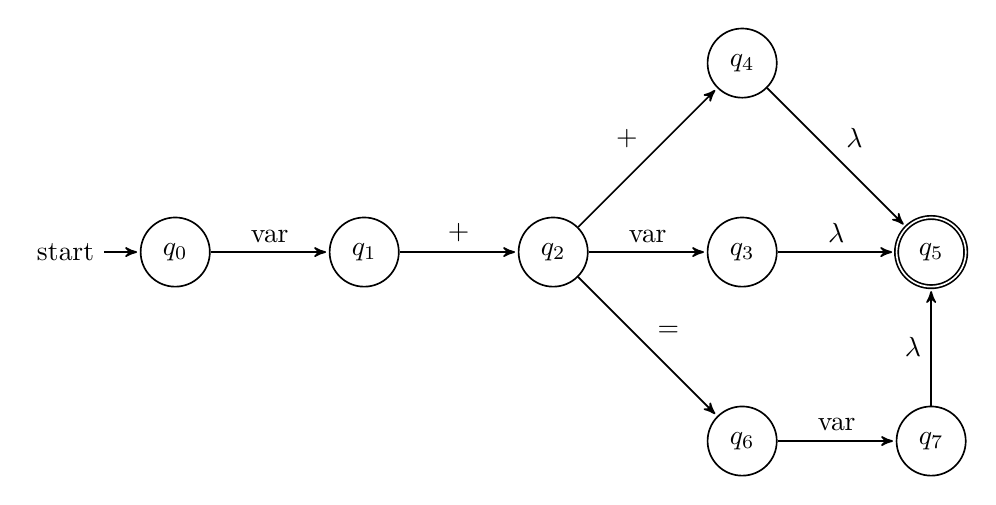
\begin{tikzpicture}[->,>=stealth',shorten >=1pt,auto,node distance=2.4cm,semithick]
  \tikzstyle{every state}=[fill=none,draw=black,text=black]

  \node[initial,state] (q0)                    {$q_0$};
  \node[state]         (q1) [right of=q0] {$q_1$};
  \node[state]         (q2) [right of=q1] {$q_2$};
  \node[state]         (q3) [right of=q2] {$q_3$};
  \node[state]         (q4) [above of=q3] {$q_4$};
  \node[state,accepting]         (q5) [right of=q3] {$q_5$};
  \node[state]         (q6) [below of=q3] {$q_6$};
  \node[state]         (q7) [below of=q5] {$q_7$};

  \path
  (q0) edge node {var} (q1)
  (q1) edge node {+} (q2)
  (q2) edge node {var} (q3)
  edge node {+} (q4)
  edge node {=} (q6)
  (q3) edge node {$\lambda$} (q5)
  (q4) edge node {$\lambda$} (q5)
  (q6) edge node {var} (q7)
  (q7) edge node {$\lambda$} (q5);
\end{tikzpicture}


% transition talbe
\begin{center}
  \begin{tabular}{ | l || c | c | c | r | }
    \hline
     & var & + & = & $\lambda$ \\ \hline \hline
    $\,\to\, q_0$ & $q_1$ & 0 & 0 & 0 \\ \hline
    $q_1$ & 0 & $q_2$ & 0 & 0 \\ \hline
    $q_2$ & $q_3$ & $q_4$ & $q_6$ & 0 \\ \hline
    $q_3$ & 0 & 0 & 0 & $q_5$ \\ \hline
    $q_4$ & 0 & 0 & 0 & $q_5$ \\ \hline
    $* q_5$ & 0 & 0 & 0 & 0 \\ \hline
    $q_6$ & $q_7$ & 0 & 0 & 0 \\ \hline
    $q_7$ & 0 & 0 & 0 & $q_5$ \\ \hline
  \end{tabular}
\end{center}

%%% Second Automata
\subsection*{var$--$, var $-$ var, var$-=$}

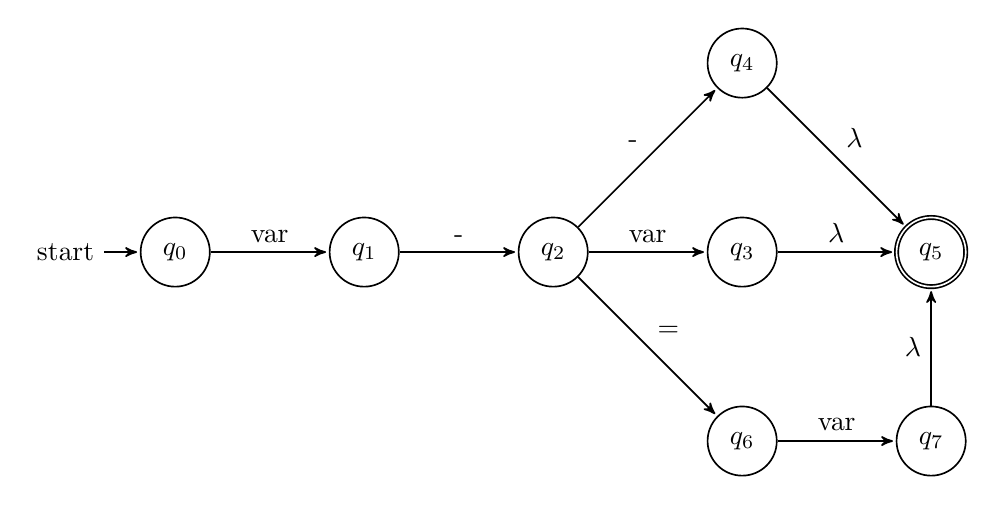
\begin{tikzpicture}[->,>=stealth',shorten >=1pt,auto,node distance=2.4cm,semithick]
  \tikzstyle{every state}=[fill=none,draw=black,text=black]

  \node[initial,state] (q0)                    {$q_0$};
  \node[state]         (q1) [right of=q0] {$q_1$};
  \node[state]         (q2) [right of=q1] {$q_2$};
  \node[state]         (q3) [right of=q2] {$q_3$};
  \node[state]         (q4) [above of=q3] {$q_4$};
  \node[state,accepting]         (q5) [right of=q3] {$q_5$};
  \node[state]         (q6) [below of=q3] {$q_6$};
  \node[state]         (q7) [below of=q5] {$q_7$};

  \path
  (q0) edge node {var} (q1)
  (q1) edge node {-} (q2)
  (q2) edge node {var} (q3)
  edge node {-} (q4)
  edge node {=} (q6)
  (q3) edge node {$\lambda$} (q5)
  (q4) edge node {$\lambda$} (q5)
  (q6) edge node {var} (q7)
  (q7) edge node {$\lambda$} (q5);
\end{tikzpicture}

% transition talbe
\begin{center}
  \begin{tabular}{ | l || c | c | c | r | }
    \hline
     & var & - & = & $\lambda$ \\ \hline \hline
    $\,\to\, q_0$ & $q_1$ & 0 & 0 & 0 \\ \hline
    $q_1$ & 0 & $q_2$ & 0 & 0 \\ \hline
    $q_2$ & $q_3$ & $q_4$ & $q_6$ & 0 \\ \hline
    $q_3$ & 0 & 0 & 0 & $q_5$ \\ \hline
    $q_4$ & 0 & 0 & 0 & $q_5$ \\ \hline
    $* q_5$ & 0 & 0 & 0 & 0 \\ \hline
    $q_6$ & $q_7$ & 0 & 0 & 0 \\ \hline
    $q_7$ & 0 & 0 & 0 & $q_5$ \\ \hline
  \end{tabular}
\end{center}

\subsection*{var * var, var*=}

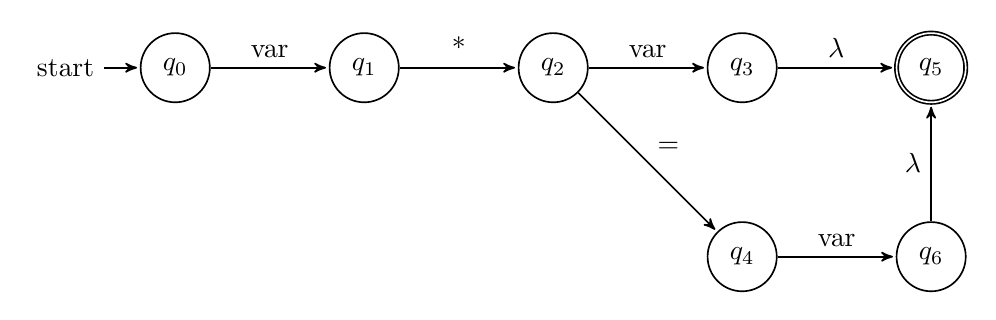
\begin{tikzpicture}[->,>=stealth',shorten >=1pt,auto,node distance=2.4cm,semithick]
  \tikzstyle{every state}=[fill=none,draw=black,text=black]

  \node[initial,state] (q0)                    {$q_0$};
  \node[state]         (q1) [right of=q0] {$q_1$};
  \node[state]         (q2) [right of=q1] {$q_2$};
  \node[state]         (q3) [right of=q2] {$q_3$};
  \node[state,accepting]         (q5) [right of=q3] {$q_5$};
  \node[state]         (q4) [below of=q3] {$q_4$};
  \node[state]         (q6) [below of=q5] {$q_6$};

  \path
  (q0) edge node {var} (q1)
  (q1) edge node {*} (q2)
  (q2) edge node {var} (q3)
  edge node {=} (q4)
  (q3) edge node {$\lambda$} (q5)
  (q4) edge node {var} (q6)
  (q6) edge node {$\lambda$} (q5);
\end{tikzpicture}
% transition talbe
\begin{center}
  \begin{tabular}{ | l || c | c | c | r | }
    \hline
     & var & * & = & $\lambda$ \\ \hline \hline
    $\,\to\, q_0$ & $q_1$ & 0 & 0 & 0 \\ \hline
    $q_1$ & 0 & $q_2$ & 0 & 0 \\ \hline
    $q_2$ & $q_3$ & 0 & $q_4$ & 0 \\ \hline
    $q_3$ & 0 & 0 & 0 & $q_5$ \\ \hline
    $q_4$ & $q_6$ & 0 & 0 & 0 \\ \hline
    $* q_5$ & 0 & 0 & 0 & 0 \\ \hline
    $q_6$ & 0 & 0 & 0 &  $q_5$ \\ \hline
  \end{tabular}
\end{center}
\subsection*{var / var, var/=}

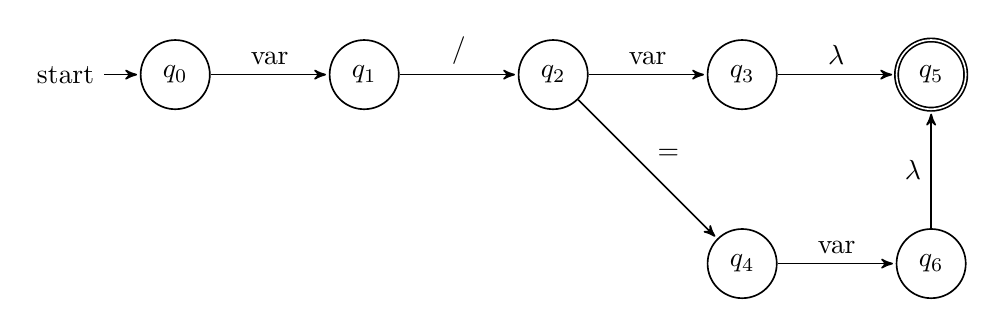
\begin{tikzpicture}[->,>=stealth',shorten >=1pt,auto,node distance=2.4cm,semithick]
  \tikzstyle{every state}=[fill=none,draw=black,text=black]

  \node[initial,state] (q0)                    {$q_0$};
  \node[state]         (q1) [right of=q0] {$q_1$};
  \node[state]         (q2) [right of=q1] {$q_2$};
  \node[state]         (q3) [right of=q2] {$q_3$};
  \node[state,accepting]         (q5) [right of=q3] {$q_5$};
  \node[state]         (q4) [below of=q3] {$q_4$};
  \node[state]         (q6) [below of=q5] {$q_6$};

  \path
  (q0) edge node {var} (q1)
  (q1) edge node {/} (q2)
  (q2) edge node {var} (q3)
  edge node {=} (q4)
  (q3) edge node {$\lambda$} (q5)
  (q4) edge node {var} (q6)
  (q6) edge node {$\lambda$} (q5);
\end{tikzpicture}
% transition talbe
\begin{center}
  \begin{tabular}{ | l || c | c | c | r | }
    \hline
     & var & / & = & $\lambda$ \\ \hline \hline
    $\,\to\, q_0$ & $q_1$ & 0 & 0 & 0 \\ \hline
    $q_1$ & 0 & $q_2$ & 0 & 0 \\ \hline
    $q_2$ & $q_3$ & 0 & $q_4$ & 0 \\ \hline
    $q_3$ & 0 & 0 & 0 & $q_5$ \\ \hline
    $q_4$ & $q_6$ & 0 & 0 & 0 \\ \hline
    $* q_5$ & 0 & 0 & 0 & 0 \\ \hline
    $q_6$ & 0 & 0 & 0 &  $q_5$ \\ \hline
  \end{tabular}
\end{center}

\subsection*{var \% var, var\%=}

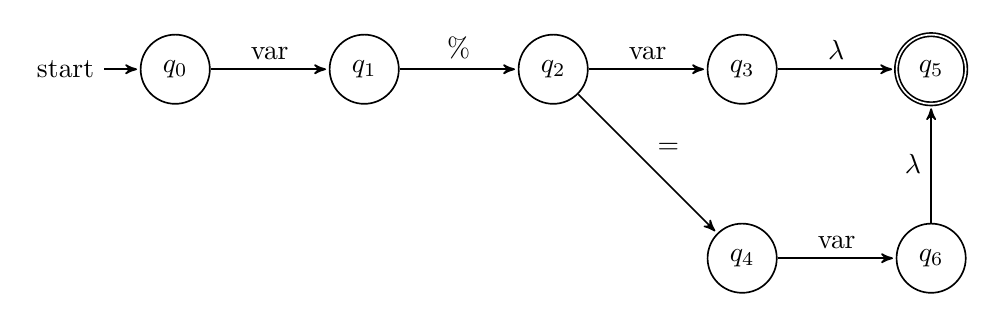
\begin{tikzpicture}[->,>=stealth',shorten >=1pt,auto,node distance=2.4cm,semithick]
  \tikzstyle{every state}=[fill=none,draw=black,text=black]

  \node[initial,state] (q0)                    {$q_0$};
  \node[state]         (q1) [right of=q0] {$q_1$};
  \node[state]         (q2) [right of=q1] {$q_2$};
  \node[state]         (q3) [right of=q2] {$q_3$};
  \node[state,accepting]         (q5) [right of=q3] {$q_5$};
  \node[state]         (q4) [below of=q3] {$q_4$};
  \node[state]         (q6) [below of=q5] {$q_6$};

  \path
  (q0) edge node {var} (q1)
  (q1) edge node {\%} (q2)
  (q2) edge node {var} (q3)
  edge node {=} (q4)
  (q3) edge node {$\lambda$} (q5)
  (q4) edge node {var} (q6)
  (q6) edge node {$\lambda$} (q5);
\end{tikzpicture}

% transition talbe
\begin{center}
  \begin{tabular}{ | l || c | c | c | r | }
    \hline
    & var & \% & = & $\lambda$ \\ \hline \hline
   $\,\to\, q_0$ & $q_1$ & 0 & 0 & 0 \\ \hline
   $q_1$ & 0 & $q_2$ & 0 & 0 \\ \hline
   $q_2$ & $q_3$ & 0 & $q_4$ & 0 \\ \hline
   $q_3$ & 0 & 0 & 0 & $q_5$ \\ \hline
   $q_4$ & $q_6$ & 0 & 0 & 0 \\ \hline
   $* q_5$ & 0 & 0 & 0 & 0 \\ \hline
    $q_6$ & 0 & 0 & 0 &  $q_5$ \\ \hline
\end{tabular}
\end{center}


\subsection*{var\&\&, var \& var, var\&=}

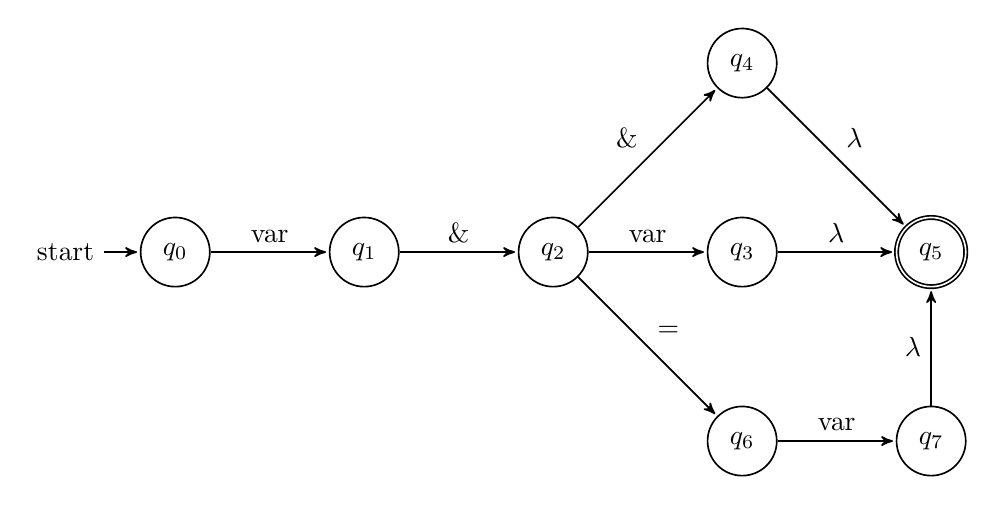
\begin{tikzpicture}[->,>=stealth',shorten >=1pt,auto,node distance=2.4cm,semithick]
  \tikzstyle{every state}=[fill=none,draw=black,text=black]

  \node[initial,state] (q0)                    {$q_0$};
  \node[state]         (q1) [right of=q0] {$q_1$};
  \node[state]         (q2) [right of=q1] {$q_2$};
  \node[state]         (q3) [right of=q2] {$q_3$};
  \node[state]         (q4) [above of=q3] {$q_4$};
  \node[state,accepting]         (q5) [right of=q3] {$q_5$};
  \node[state]         (q6) [below of=q3] {$q_6$};
  \node[state]         (q7) [below of=q5] {$q_7$};

  \path
  (q0) edge node {var} (q1)
  (q1) edge node {\&} (q2)
  (q2) edge node {var} (q3)
  edge node {\&} (q4)
  edge node {=} (q6)
  (q3) edge node {$\lambda$} (q5)
  (q4) edge node {$\lambda$} (q5)
  (q6) edge node {var} (q7)
  (q7) edge node {$\lambda$} (q5);
\end{tikzpicture}

% transition talbe
\begin{center}
  \begin{tabular}{ | l || c | c | c | r | }
    \hline
     & var & \& & = & $\lambda$ \\ \hline \hline
    $\,\to\, q_0$ & $q_1$ & 0 & 0 & 0 \\ \hline
    $q_1$ & 0 & $q_2$ & 0 & 0 \\ \hline
    $q_2$ & $q_3$ & $q_4$ & $q_6$ & 0 \\ \hline
    $q_3$ & 0 & 0 & 0 & $q_5$ \\ \hline
    $q_4$ & 0 & 0 & 0 & $q_5$ \\ \hline
    $* q_5$ & 0 & 0 & 0 & 0 \\ \hline
    $q_6$ & $q_7$ & 0 & 0 & 0 \\ \hline
    $q_7$ & 0 & 0 & 0 & $q_5$ \\ \hline
  \end{tabular}
\end{center}


\subsection*{var$||$, var $|$ var, var$|$=}

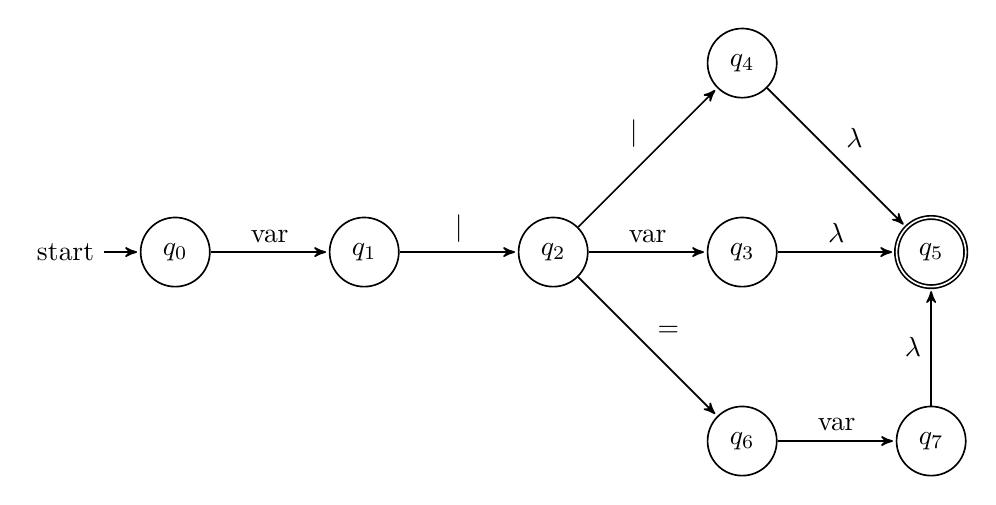
\begin{tikzpicture}[->,>=stealth',shorten >=1pt,auto,node distance=2.4cm,semithick]
  \tikzstyle{every state}=[fill=none,draw=black,text=black]

  \node[initial,state] (q0)                    {$q_0$};
  \node[state]         (q1) [right of=q0] {$q_1$};
  \node[state]         (q2) [right of=q1] {$q_2$};
  \node[state]         (q3) [right of=q2] {$q_3$};
  \node[state]         (q4) [above of=q3] {$q_4$};
  \node[state,accepting]         (q5) [right of=q3] {$q_5$};
  \node[state]         (q6) [below of=q3] {$q_6$};
  \node[state]         (q7) [below of=q5] {$q_7$};

  \path
  (q0) edge node {var} (q1)
  (q1) edge node {$|$} (q2)
  (q2) edge node {var} (q3)
  edge node {$|$} (q4)
  edge node {=} (q6)
  (q3) edge node {$\lambda$} (q5)
  (q4) edge node {$\lambda$} (q5)
  (q6) edge node {var} (q7)
  (q7) edge node {$\lambda$} (q5);
\end{tikzpicture}

% transition talbe
\begin{center}
  \begin{tabular}{ | l || c | c | c | r | }
   \hline
    & var & $|$ & = & $\lambda$ \\ \hline \hline
   $\,\to\, q_0$ & $q_1$ & 0 & 0 & 0 \\ \hline
   $q_1$ & 0 & $q_2$ & 0 & 0 \\ \hline
   $q_2$ & $q_3$ & $q_4$ & $q_6$ & 0 \\ \hline
   $q_3$ & 0 & 0 & 0 & $q_5$ \\ \hline
   $q_4$ & 0 & 0 & 0 & $q_5$ \\ \hline
   $* q_5$ & 0 & 0 & 0 & 0 \\ \hline
   $q_6$ & $q_7$ & 0 & 0 & 0 \\ \hline
    $q_7$ & 0 & 0 & 0 & $q_5$ \\ \hline
  \end{tabular}
\end{center}



\subsection*{var \^{} var, var\^{}=}

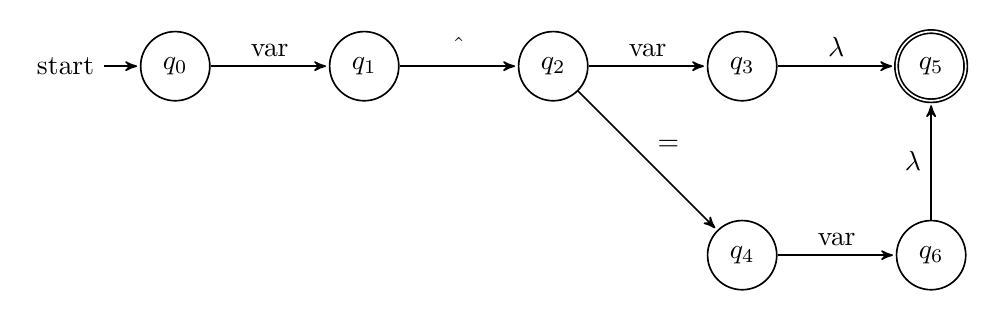
\begin{tikzpicture}[->,>=stealth',shorten >=1pt,auto,node distance=2.4cm,semithick]
  \tikzstyle{every state}=[fill=none,draw=black,text=black]

  \node[initial,state] (q0)                    {$q_0$};
  \node[state]         (q1) [right of=q0] {$q_1$};
  \node[state]         (q2) [right of=q1] {$q_2$};
  \node[state]         (q3) [right of=q2] {$q_3$};
  \node[state,accepting]         (q5) [right of=q3] {$q_5$};
  \node[state]         (q4) [below of=q3] {$q_4$};
  \node[state]         (q6) [below of=q5] {$q_6$};

  \path
  (q0) edge node {var} (q1)
  (q1) edge node {\^{}} (q2)
  (q2) edge node {var} (q3)
  edge node {=} (q4)
  (q3) edge node {$\lambda$} (q5)
  (q4) edge node {var} (q6)
  (q6) edge node {$\lambda$} (q5);
\end{tikzpicture}

% transition talbe
\begin{center}
  \begin{tabular}{ | l || c | c | c | r | }
    \hline
     & var & \^{} & = & $\lambda$ \\ \hline \hline
    $\,\to\, q_0$ & $q_1$ & 0 & 0 & 0 \\ \hline
    $q_1$ & 0 & $q_2$ & 0 & 0 \\ \hline
    $q_2$ & $q_3$ & 0 & $q_4$ & 0 \\ \hline
    $q_3$ & 0 & 0 & 0 & $q_5$ \\ \hline
    $q_4$ & $q_6$ & 0 & 0 & 0 \\ \hline
    $* q_5$ & 0 & 0 & 0 & 0 \\ \hline
    $q_6$ & 0 & 0 & 0 &  $q_5$ \\ \hline
 \end{tabular}
\end{center}


\subsection*{var $<$ var, var $<=$ var, var $<<$ var, var $<<=$ var}

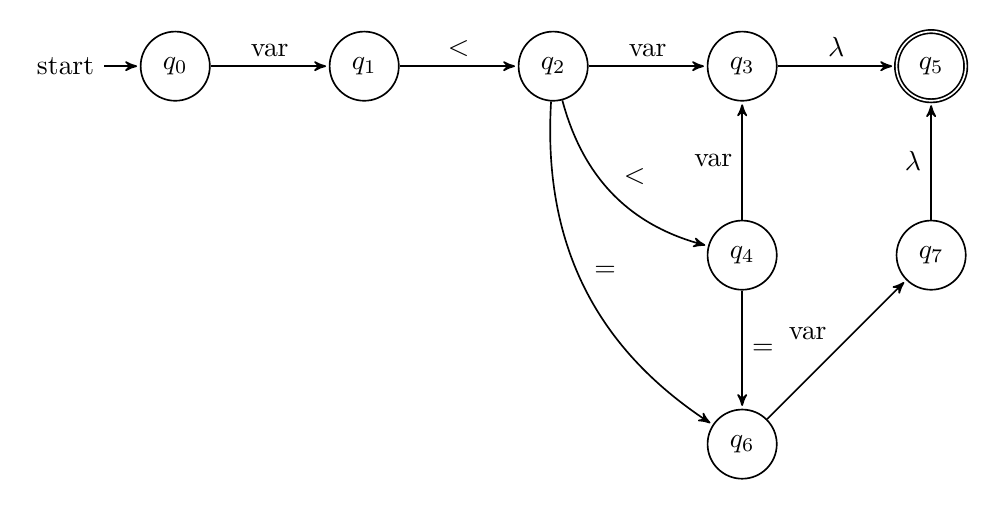
\begin{tikzpicture}[->,>=stealth',shorten >=1pt,auto,node distance=2.4cm,semithick]
  \tikzstyle{every state}=[fill=none,draw=black,text=black]

  \node[initial,state] (q0)                    {$q_0$};
  \node[state]         (q1) [right of=q0] {$q_1$};
  \node[state]         (q2) [right of=q1] {$q_2$};
  \node[state]         (q3) [right of=q2] {$q_3$};
  \node[state]         (q4) [below of=q3] {$q_4$};
  \node[state,accepting]         (q5) [right of=q3] {$q_5$};
  \node[state]         (q6) [below of=q4] {$q_6$};
  \node[state]         (q7) [below of=q5] {$q_7$};

  \path
  (q0) edge node {var} (q1)
  (q1) edge node {$<$} (q2)
  (q2) edge node {var} (q3)
  edge [bend right] node {$<$} (q4)
  edge [bend right] node {=} (q6)
  (q3) edge node {$\lambda$} (q5)
  (q4) edge node {var} (q3)
  edge node {$=$} (q6)
  (q6) edge node {var} (q7)
  (q7) edge node {$\lambda$} (q5);
\end{tikzpicture}

% transition talbe
\begin{center}
  \begin{tabular}{ | l || c | c | c | r | }
    \hline
     & var & $<$ & = & $\lambda$ \\ \hline \hline
    $\,\to\, q_0$ & $q_1$ & 0 & 0 & 0 \\ \hline
    $q_1$ & 0 & $q_2$ & 0 & 0 \\ \hline
    $q_2$ & $q_3$ & $q_4$ & $q_6$ & 0 \\ \hline
    $q_3$ & 0 & 0 & 0 & $q_5$ \\ \hline
    $q_4$ & $q_3$ & 0 &  $q_6$ & 0 \\ \hline
    $* q_5$ & 0 & 0 & 0 & 0 \\ \hline
    $q_6$ & $q_7$ & 0 & 0 & 0 \\ \hline
    $q_7$ & 0 & 0 & 0 & $q_5$ \\ \hline
  \end{tabular}
\end{center}

\subsection*{var $>$ var, var $>=$ var, var $>>$ var, var $>>=$ var, var $>>>=$ var}

\begin{tikzpicture}[->,>=stealth',shorten >=1pt,auto,node distance=3cm,semithick]
  \tikzstyle{every state}=[fill=none,draw=black,text=black]

  \node[initial,state] (q0)                    {$q_0$};
  \node[state]         (q1) [right of=q0] {$q_1$};
  \node[state]         (q2) [right of=q1] {$q_2$};
  \node[state]         (q3) [right of=q2] {$q_3$};
  \node[state]         (q4) [below of=q3] {$q_4$};
  \node[state,accepting]         (q5) [right of=q3] {$q_5$};
  \node[state]         (q6) [below of=q4] {$q_6$};
  \node[state]         (q7) [below of=q5] {$q_7$};
  \node[state]         (q8) [below of=q6] {$q_8$};
  

  \path
  (q0) edge node {var} (q1)
  (q1) edge node {$>$} (q2)
  (q2) edge node {var} (q3)
  edge [bend right] node {$>$} (q4)
  edge [bend right] node {=} (q8)
  (q3) edge node {$\lambda$} (q5)
  (q4) edge node {var} (q3)
  edge node {$>$} (q6)
  edge [bend right] node {$=$} (q8)
  (q6) edge node {=} (q8)
  (q8) edge node {var} (q7)
  (q7) edge node {$\lambda$} (q5);
\end{tikzpicture}

% transition talbe
\begin{center}
  \begin{tabular}{ | l || c | c | c | r | }
    \hline
     & var & $>$ & = & $\lambda$ \\ \hline \hline
    $\,\to\, q_0$ & $q_1$ & 0 & 0 & 0 \\ \hline
    $q_1$ & 0 & $q_2$ & 0 & 0 \\ \hline
    $q_2$ & $q_3$ & $q_4$ & $q_6$ & 0 \\ \hline
    $q_3$ & 0 & 0 & 0 & $q_5$ \\ \hline
    $q_4$ & $q_3$ & $q_6$ & $q_8$ & 0 \\ \hline
    $* q_5$ & 0 & 0 & 0 & 0 \\ \hline
    $q_6$ & $q_7$ & 0 & $q_8$ & 0 \\ \hline
    $q_7$ & 0 & 0 & 0 & $q_5$ \\ \hline
    $q_8$ &  $q_7$ & 0 & 0 & 0 \\ \hline
  \end{tabular}
\end{center}
 

\subsection*{var $==$ var, var $!=$ var}

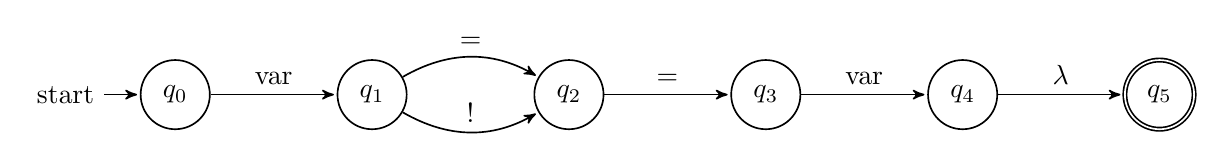
\begin{tikzpicture}[->,>=stealth',shorten >=1pt,auto,node distance=2.5cm,semithick]
  \tikzstyle{every state}=[fill=none,draw=black,text=black]

  \node[initial,state] (q0)                    {$q_0$};
  \node[state]         (q1) [right of=q0] {$q_1$};
  \node[state]         (q2) [right of=q1] {$q_2$};
  \node[state]         (q3) [right of=q2] {$q_3$};
  \node[state]         (q4) [right of=q3] {$q_4$};
  \node[state, accepting]         (q5) [right of=q4] {$q_5$};

  \path
  (q0) edge node {var} (q1)
  (q1) edge [bend left] node {=} (q2)
  edge [bend right] node {!} (q2)
  (q2) edge node {=} (q3)
  (q3) edge node {var} (q4)
  (q4) edge node {$\lambda$} (q5);
\end{tikzpicture}
% transition talbe
\begin{center}
  \begin{tabular}{ | l || c | c | c | r | }
    \hline
     & var & !  & = & $\lambda$ \\ \hline \hline
    $\,\to\, q_0$ & $q_1$ & 0 & 0 & 0 \\ \hline
    $q_1$ & 0 & $q_2$ &  $q_2$ & 0 \\ \hline
    $q_2$ & 0 & 0 &  $q_3$ & 0 \\ \hline
    $q_3$ &  $q_4$ & 0 & 0 & 0 \\ \hline
    $q_4$ & 0 & 0 & 0 &  $q_5$ \\ \hline
    $* q_5$ & 0 & 0 & 0 & 0 \\ \hline
  \end{tabular}
\end{center}



\subsection*{$++$var, $+$var}

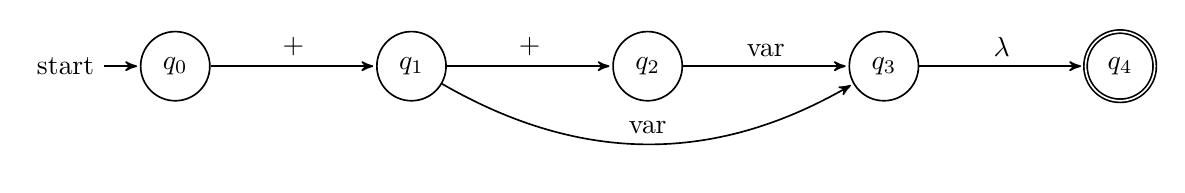
\begin{tikzpicture}[->,>=stealth',shorten >=1pt,auto,node distance=3cm,semithick]
  \tikzstyle{every state}=[fill=none,draw=black,text=black]

  \node[initial,state] (q0)                    {$q_0$};
  \node[state]         (q1) [right of=q0] {$q_1$};
  \node[state]         (q2) [right of=q1] {$q_2$};
  \node[state]         (q3) [right of=q2] {$q_3$};
  \node[state, accepting]         (q4) [right of=q3] {$q_4$};

  \path
  (q0) edge node {+} (q1)
  (q1) edge node {+} (q2)
  edge [bend right] node {var} (q3)
  (q2) edge node {var} (q3)
  (q3) edge node {$\lambda$} (q4);
\end{tikzpicture}

% transition talbe error
\begin{center}
  \begin{tabular}{ | l || c | c | r | }
    \hline
     & var & +  & $\lambda$ \\ \hline \hline
    $\,\to\, q_0$ & $q_1$ & 0  & 0 \\ \hline
    $q_1$  & $q_2$ &  $q_2$ & 0 \\ \hline
    $q_2$  &  $q_3$  &  $q_3$ & 0 \\ \hline
    $q_3$ &  $q_4$  & 0 & 0 \\ \hline
    $*q_4$ & 0  & 0 & 0 \\ \hline
   
  \end{tabular}
\end{center}
 

\subsection*{$--$var, $-$var}

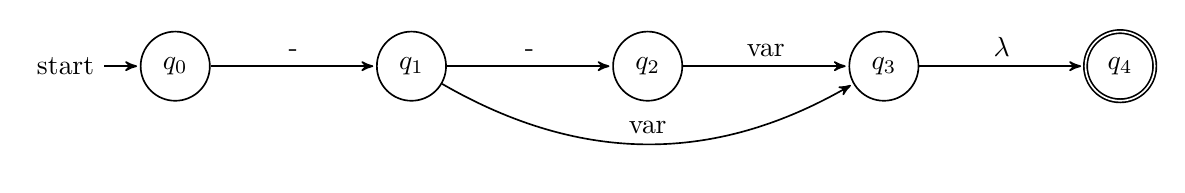
\begin{tikzpicture}[->,>=stealth',shorten >=1pt,auto,node distance=3cm,semithick]
  \tikzstyle{every state}=[fill=none,draw=black,text=black]

  \node[initial,state] (q0)                    {$q_0$};
  \node[state]         (q1) [right of=q0] {$q_1$};
  \node[state]         (q2) [right of=q1] {$q_2$};
  \node[state]         (q3) [right of=q2] {$q_3$};
  \node[state, accepting]         (q4) [right of=q3] {$q_4$};

  \path
  (q0) edge node {-} (q1)
  (q1) edge node {-} (q2)
  edge [bend right] node {var} (q3)
  (q2) edge node {var} (q3)
  (q3) edge node {$\lambda$} (q4);
\end{tikzpicture}

% transition talbe
\begin{center}
  \begin{tabular}{ | l || c | c | r | }
    \hline
     & var & - & $\lambda$ \\ \hline \hline
    $\,\to\, q_0$ & $q_1$ & 0 & 0  \\ \hline
    $q_1$ & 0 & $q_2$ & $q_2$  \\ \hline
    $q_2$ & 0 &  $q_3$  & $q_3$  \\ \hline
    $q_3$ &  $q_4$  & 0 & 0 \\ \hline
    $*q_4$ & 0 & 0 & 0 \\ \hline
   
  \end{tabular}
\end{center}


\subsection*{$!$ var}

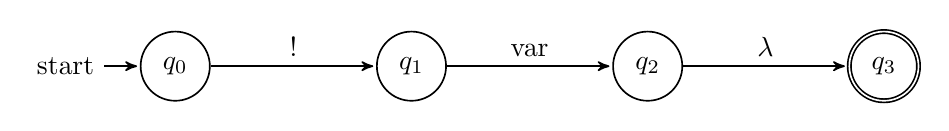
\begin{tikzpicture}[->,>=stealth',shorten >=1pt,auto,node distance=3cm,semithick]
  \tikzstyle{every state}=[fill=none,draw=black,text=black]

  \node[initial,state] (q0)                    {$q_0$};
  \node[state]         (q1) [right of=q0] {$q_1$};
  \node[state]         (q2) [right of=q1] {$q_2$};
  \node[state, accepting]         (q3) [right of=q2] {$q_3$};

  \path
  (q0) edge node {$!$} (q1)
  (q1) edge node {var} (q2)
  (q2) edge node {$\lambda$} (q3);
\end{tikzpicture}

% transition talbe
\begin{center}
  \begin{tabular}{ | l || c | c | r | }
    \hline
     & var & ! & $\lambda$ \\ \hline \hline
    $\,\to\, q_0$ & 0 &  $q_1$  & 0 \\ \hline
    $q_1$ & $q_2$ & 0  & 0 \\ \hline
    $q_2$ & 0 & 0 & $q_3$ \\ \hline
    $*q_3$ &  0 & 0 & 0 \\ \hline
      
  \end{tabular}
\end{center}


\subsection*{$\sim$ var}

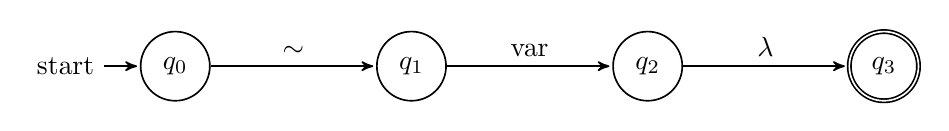
\begin{tikzpicture}[->,>=stealth',shorten >=1pt,auto,node distance=3cm,semithick]
  \tikzstyle{every state}=[fill=none,draw=black,text=black]

  \node[initial,state] (q0)                    {$q_0$};
  \node[state]         (q1) [right of=q0] {$q_1$};
  \node[state]         (q2) [right of=q1] {$q_2$};
  \node[state, accepting]         (q3) [right of=q2] {$q_3$};

  \path
  (q0) edge node {$\sim$} (q1)
  (q1) edge node {var} (q2)
  (q2) edge node {$\lambda$} (q3);
\end{tikzpicture}

% transition talbe
\begin{center}
  \begin{tabular}{ | l || c | c | r | }
    \hline
     & var & $\sim$ & $\lambda$ \\ \hline \hline
    $\,\to\, q_0$ & 0 &  $q_1$  & 0 \\ \hline
    $q_1$ & $q_2$ & 0  & 0 \\ \hline
    $q_2$ & 0 & 0 & $q_3$ \\ \hline
    $*q_3$ &  0 & 0 & 0 \\ \hline
      
  \end{tabular}
\end{center}

\subsection*{condition ? statement : statement}

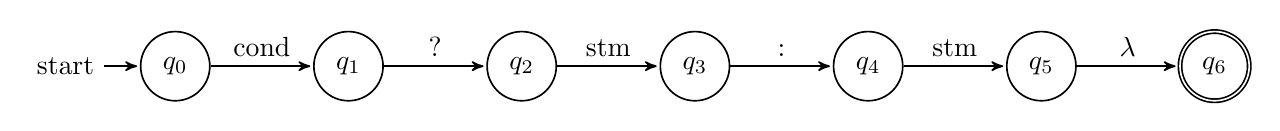
\begin{tikzpicture}[->,>=stealth',shorten >=1pt,auto,node distance=2.2cm,semithick]
  \tikzstyle{every state}=[fill=none,draw=black,text=black]

  \node[initial,state] (q0)                    {$q_0$};
  \node[state]         (q1) [right of=q0] {$q_1$};
  \node[state]         (q2) [right of=q1] {$q_2$};
  \node[state]         (q3) [right of=q2] {$q_3$};
  \node[state]         (q4) [right of=q3] {$q_4$};
  \node[state]         (q5) [right of=q4] {$q_5$};
  \node[state, accepting]         (q6) [right of=q5] {$q_6$};

  \path
  (q0) edge node {cond} (q1)
  (q1) edge node {?} (q2)
  (q2) edge node {stm} (q3)
  (q3) edge node {:} (q4)
  (q4) edge node {stm} (q5)
  (q5) edge node {$\lambda$} (q6);
\end{tikzpicture}

\section*{Operadores de Java}

\begin{center}
  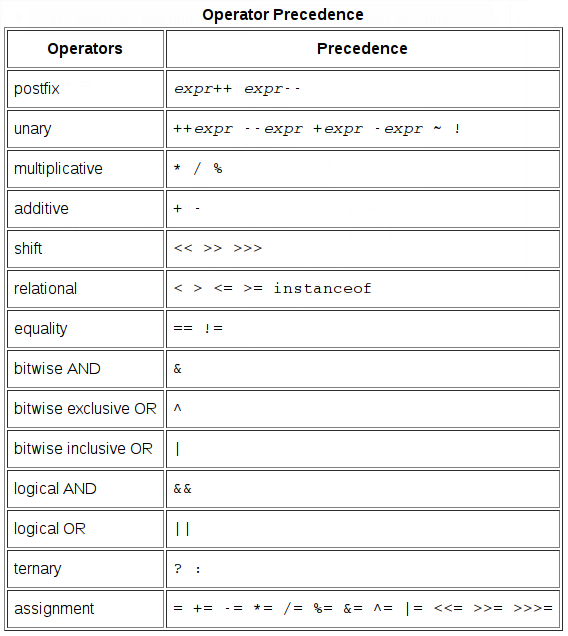
\includegraphics[scale=0.5]{java_operators}
\end{center}

Esta información fue obtenida de la documentación ofical de Java. \cite{java}
\section*{Conclusiones }
Como una conclusión, la gramática libre de contexto podría no ser la más apropiada. No incluye en forma algunas convenciones estándar relacionadaa con la precedencia de operadores y el orden de evaluación de izquierda a derecha, que se usa para evaluar la expresión. (La precedencia de operadores indica que en la expresión a + b * c, la multiplicación se realiza antes que la suma). 

Por consiguiente, en lugar de verse en la necesidad de elegir entre dos derivaciones de una cadena es aconsejable utilizar una derivación. Siendo así la forma más sencilla de evaluar una expresión algebraica.

\begin{thebibliography}{20}
\bibitem{java} https://docs.oracle.com/javase/tutorial/java/nutsandbolts/operators.html
\end{thebibliography}

\end{document}
